%% energy_gdp_channels.tex
%% Transmission channels from energy policy to macroeconomic outcomes
%% in DGE-METRIC.  Three policy levers → model mechanisms → macro outcomes.
%% Compile with: pdflatex energy_gdp_channels.tex
\documentclass[tikz,border=14pt]{standalone}
\usepackage{tikz}
\usepackage{amsmath}
\usetikzlibrary{positioning,arrows.meta,calc,fit,backgrounds,shapes.misc}

%% ---- colour palette ---------------------------------------------------
\definecolor{Crimson}{RGB}{150,15,15}
\definecolor{CrimsonMid}{RGB}{175,45,45}
\definecolor{CoalGray}{RGB}{75,75,90}
\definecolor{ForestGreen}{RGB}{25,115,65}
\definecolor{NavyBlue}{RGB}{25,60,130}
\definecolor{AmberOrange}{RGB}{195,100,15}
\definecolor{TealBlue}{RGB}{20,110,120}
\definecolor{LightGray}{RGB}{235,235,240}

\begin{document}
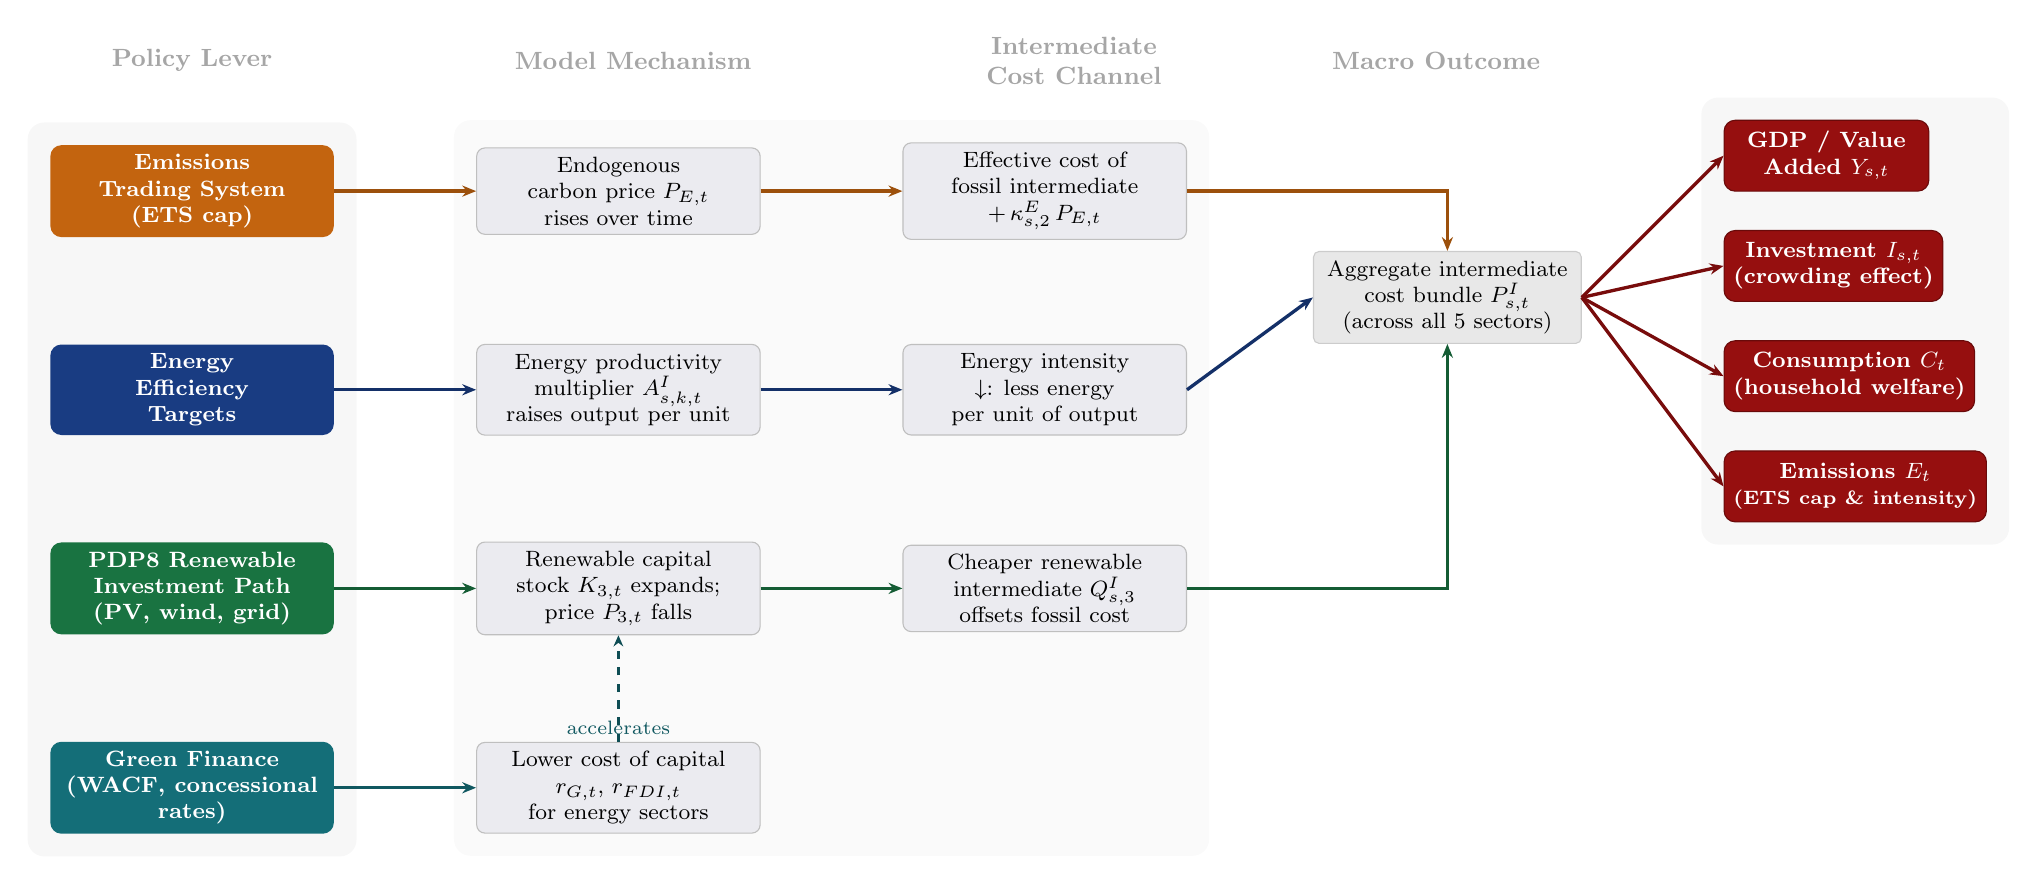
\begin{tikzpicture}[
  %% --- node styles --------------------------------------------------
  policybox/.style={
    rectangle, rounded corners=4pt,
    text=white, font=\footnotesize\bfseries,
    minimum width=3.6cm, minimum height=0.95cm,
    align=center
  },
  mechbox/.style={
    rectangle, rounded corners=3pt,
    fill=LightGray, draw=gray!50,
    font=\footnotesize,
    minimum width=3.6cm, minimum height=0.90cm,
    align=center
  },
  outbox/.style={
    rectangle, rounded corners=4pt,
    fill=Crimson, draw=Crimson!70!black,
    text=white, font=\footnotesize\bfseries,
    minimum width=2.6cm, minimum height=0.90cm,
    align=center
  },
  connector/.style={
    rectangle, rounded corners=2pt,
    fill=gray!18, draw=gray!40,
    font=\footnotesize,
    minimum width=3.4cm, minimum height=0.85cm,
    align=center
  },
  sectionlabel/.style={
    font=\small\bfseries, text=gray!70
  },
  %% --- arrow styles -------------------------------------------------
  mainarr/.style={
    -{Stealth[length=5pt,width=4pt]},
    line width=1.2pt
  },
  subarr/.style={
    -{Stealth[length=4pt,width=3.5pt]},
    line width=0.9pt, gray!70
  },
  dasharr/.style={
    -{Stealth[length=4pt,width=3.5pt]},
    line width=0.8pt, dashed, gray!70
  },
]

%% ==================================================================
%% COLUMN HEADERS
%% ==================================================================
\node[sectionlabel] (h1) at (0, 0)       {Policy Lever};
\node[sectionlabel] (h2) at (5.6, 0)     {Model Mechanism};
\node[sectionlabel, align=center] (h3) at (11.2, 0) {Intermediate\\Cost Channel};
\node[sectionlabel] (h4) at (15.8, 0)    {Macro Outcome};

%% ==================================================================
%% ROW 1 — ETS / Carbon market
%% ==================================================================
\node[policybox, fill=AmberOrange, below=0.8cm of h1] (p_ets)
  {Emissions\\Trading System\\(ETS cap)};

\node[mechbox, right=1.8cm of p_ets] (m_etsprice)
  {Endogenous\\carbon price $P_{E,t}$\\rises over time};

\node[mechbox, right=1.8cm of m_etsprice] (m_fossilcost)
  {Effective cost of\\fossil intermediate\\$+\,\kappa^E_{s,2}\,P_{E,t}$};

\draw[mainarr, AmberOrange!80!black]
  (p_ets.east) -- (m_etsprice.west);
\draw[mainarr, AmberOrange!80!black]
  (m_etsprice.east) -- (m_fossilcost.west);

%% ==================================================================
%% ROW 2 — Energy Efficiency
%% ==================================================================
\node[policybox, fill=NavyBlue, below=1.35cm of p_ets] (p_ee)
  {Energy\\Efficiency\\Targets};

\node[mechbox, right=1.8cm of p_ee] (m_eeproductivity)
  {Energy productivity\\multiplier $A^{I}_{s,k,t}$\\raises output per unit};

\node[mechbox, right=1.8cm of m_eeproductivity] (m_intensdown)
  {Energy intensity\\$\downarrow$: less energy\\per unit of output};

\draw[mainarr, NavyBlue!80!black]
  (p_ee.east) -- (m_eeproductivity.west);
\draw[mainarr, NavyBlue!80!black]
  (m_eeproductivity.east) -- (m_intensdown.west);

%% ==================================================================
%% ROW 3 — Renewable Investment
%% ==================================================================
\node[policybox, fill=ForestGreen, below=1.35cm of p_ee] (p_renew)
  {PDP8 Renewable\\Investment Path\\(PV, wind, grid)};

\node[mechbox, right=1.8cm of p_renew] (m_renewcap)
  {Renewable capital\\stock $K_{3,t}$ expands;\\price $P_{3,t}$ falls};

\node[mechbox, right=1.8cm of m_renewcap] (m_renewcost)
  {Cheaper renewable\\intermediate $Q^{I}_{s,3}$\\offsets fossil cost};

\draw[mainarr, ForestGreen!80!black]
  (p_renew.east) -- (m_renewcap.west);
\draw[mainarr, ForestGreen!80!black]
  (m_renewcap.east) -- (m_renewcost.west);

%% ==================================================================
%% ROW 4 — Green Finance (lower row, feeds into row 3)
%% ==================================================================
\node[policybox, fill=TealBlue, below=1.35cm of p_renew] (p_fin)
  {Green Finance\\(WACF, concessional\\rates)};

\node[mechbox, right=1.8cm of p_fin] (m_wacc)
  {Lower cost of capital\\$r_{G,t}$, $r_{FDI,t}$\\for energy sectors};

\draw[mainarr, TealBlue!80!black]
  (p_fin.east) -- (m_wacc.west);

%% finance feeds into renewable capital
\draw[dasharr, TealBlue!70!black]
  (m_wacc.north) -- ++(0,0.4) -| (m_renewcap.south)
  node[midway, below, font=\scriptsize, text=TealBlue!80!black]
  {accelerates};

%% ==================================================================
%% INTERMEDIATE COST AGGREGATION NODE
%% ==================================================================
\node[connector,
  right=1.6cm of m_fossilcost,
  yshift=-1.35cm
] (agg) {Aggregate intermediate\\cost bundle $P^I_{s,t}$\\(across all 5 sectors)};

%% arrows from the three mechanism rows into aggregator
\draw[mainarr, AmberOrange!80!black]
  (m_fossilcost.east) -| (agg.north);
\draw[mainarr, NavyBlue!80!black]
  (m_intensdown.east) -- (agg.west);
\draw[mainarr, ForestGreen!80!black]
  (m_renewcost.east) -| (agg.south);

%% ==================================================================
%% MACRO OUTCOME BOXES  (right column)
%% ==================================================================
\node[outbox, right=1.8cm of agg, yshift=+1.8cm]  (o_gdp)
  {GDP / Value\\Added $Y_{s,t}$};

\node[outbox, right=1.8cm of agg, yshift=+0.4cm]  (o_inv)
  {Investment $I_{s,t}$\\(crowding effect)};

\node[outbox, right=1.8cm of agg, yshift=-1.0cm]  (o_cons)
  {Consumption $C_t$\\(household welfare)};

\node[outbox, right=1.8cm of agg, yshift=-2.4cm]  (o_emis)
  {Emissions $E_t$\\{\scriptsize(ETS cap \& intensity)}};

%% arrows from aggregator to outcomes
\foreach \nd in {o_gdp, o_inv, o_cons, o_emis}{
  \draw[mainarr, Crimson!80!black]
    (agg.east) -- (\nd.west);
}

%% ==================================================================
%% BACKGROUND BANDS (faint) to visually group columns
%% ==================================================================
\begin{scope}[on background layer]
  %% Policy lever band
  \node[fill=gray!06, rounded corners=6pt,
    fit=(p_ets)(p_ee)(p_renew)(p_fin), inner sep=8pt] {};
  %% Mechanism band
  \node[fill=gray!04, rounded corners=6pt,
    fit=(m_etsprice)(m_eeproductivity)(m_renewcap)(m_wacc)(m_fossilcost)(m_intensdown)(m_renewcost),
    inner sep=8pt] {};
  %% Outcome band
  \node[fill=gray!06, rounded corners=6pt,
    fit=(o_gdp)(o_inv)(o_cons)(o_emis), inner sep=8pt] {};
\end{scope}

%% (binding cap note now embedded in o_emis label above)

\end{tikzpicture}
\end{document}
